% Options for packages loaded elsewhere
\PassOptionsToPackage{unicode}{hyperref}
\PassOptionsToPackage{hyphens}{url}
%
\documentclass[
]{article}
\usepackage{lmodern}
\usepackage{amssymb,amsmath}
\usepackage{ifxetex,ifluatex}
\ifnum 0\ifxetex 1\fi\ifluatex 1\fi=0 % if pdftex
  \usepackage[T1]{fontenc}
  \usepackage[utf8]{inputenc}
  \usepackage{textcomp} % provide euro and other symbols
\else % if luatex or xetex
  \usepackage{unicode-math}
  \defaultfontfeatures{Scale=MatchLowercase}
  \defaultfontfeatures[\rmfamily]{Ligatures=TeX,Scale=1}
\fi
% Use upquote if available, for straight quotes in verbatim environments
\IfFileExists{upquote.sty}{\usepackage{upquote}}{}
\IfFileExists{microtype.sty}{% use microtype if available
  \usepackage[]{microtype}
  \UseMicrotypeSet[protrusion]{basicmath} % disable protrusion for tt fonts
}{}
\makeatletter
\@ifundefined{KOMAClassName}{% if non-KOMA class
  \IfFileExists{parskip.sty}{%
    \usepackage{parskip}
  }{% else
    \setlength{\parindent}{0pt}
    \setlength{\parskip}{6pt plus 2pt minus 1pt}}
}{% if KOMA class
  \KOMAoptions{parskip=half}}
\makeatother
\usepackage{xcolor}
\IfFileExists{xurl.sty}{\usepackage{xurl}}{} % add URL line breaks if available
\IfFileExists{bookmark.sty}{\usepackage{bookmark}}{\usepackage{hyperref}}
\hypersetup{
  pdftitle={STAT 33B Homework 4},
  pdfauthor={Ming Fong (3035619833)},
  hidelinks,
  pdfcreator={LaTeX via pandoc}}
\urlstyle{same} % disable monospaced font for URLs
\usepackage[margin=1in]{geometry}
\usepackage{color}
\usepackage{fancyvrb}
\newcommand{\VerbBar}{|}
\newcommand{\VERB}{\Verb[commandchars=\\\{\}]}
\DefineVerbatimEnvironment{Highlighting}{Verbatim}{commandchars=\\\{\}}
% Add ',fontsize=\small' for more characters per line
\usepackage{framed}
\definecolor{shadecolor}{RGB}{248,248,248}
\newenvironment{Shaded}{\begin{snugshade}}{\end{snugshade}}
\newcommand{\AlertTok}[1]{\textcolor[rgb]{0.94,0.16,0.16}{#1}}
\newcommand{\AnnotationTok}[1]{\textcolor[rgb]{0.56,0.35,0.01}{\textbf{\textit{#1}}}}
\newcommand{\AttributeTok}[1]{\textcolor[rgb]{0.77,0.63,0.00}{#1}}
\newcommand{\BaseNTok}[1]{\textcolor[rgb]{0.00,0.00,0.81}{#1}}
\newcommand{\BuiltInTok}[1]{#1}
\newcommand{\CharTok}[1]{\textcolor[rgb]{0.31,0.60,0.02}{#1}}
\newcommand{\CommentTok}[1]{\textcolor[rgb]{0.56,0.35,0.01}{\textit{#1}}}
\newcommand{\CommentVarTok}[1]{\textcolor[rgb]{0.56,0.35,0.01}{\textbf{\textit{#1}}}}
\newcommand{\ConstantTok}[1]{\textcolor[rgb]{0.00,0.00,0.00}{#1}}
\newcommand{\ControlFlowTok}[1]{\textcolor[rgb]{0.13,0.29,0.53}{\textbf{#1}}}
\newcommand{\DataTypeTok}[1]{\textcolor[rgb]{0.13,0.29,0.53}{#1}}
\newcommand{\DecValTok}[1]{\textcolor[rgb]{0.00,0.00,0.81}{#1}}
\newcommand{\DocumentationTok}[1]{\textcolor[rgb]{0.56,0.35,0.01}{\textbf{\textit{#1}}}}
\newcommand{\ErrorTok}[1]{\textcolor[rgb]{0.64,0.00,0.00}{\textbf{#1}}}
\newcommand{\ExtensionTok}[1]{#1}
\newcommand{\FloatTok}[1]{\textcolor[rgb]{0.00,0.00,0.81}{#1}}
\newcommand{\FunctionTok}[1]{\textcolor[rgb]{0.00,0.00,0.00}{#1}}
\newcommand{\ImportTok}[1]{#1}
\newcommand{\InformationTok}[1]{\textcolor[rgb]{0.56,0.35,0.01}{\textbf{\textit{#1}}}}
\newcommand{\KeywordTok}[1]{\textcolor[rgb]{0.13,0.29,0.53}{\textbf{#1}}}
\newcommand{\NormalTok}[1]{#1}
\newcommand{\OperatorTok}[1]{\textcolor[rgb]{0.81,0.36,0.00}{\textbf{#1}}}
\newcommand{\OtherTok}[1]{\textcolor[rgb]{0.56,0.35,0.01}{#1}}
\newcommand{\PreprocessorTok}[1]{\textcolor[rgb]{0.56,0.35,0.01}{\textit{#1}}}
\newcommand{\RegionMarkerTok}[1]{#1}
\newcommand{\SpecialCharTok}[1]{\textcolor[rgb]{0.00,0.00,0.00}{#1}}
\newcommand{\SpecialStringTok}[1]{\textcolor[rgb]{0.31,0.60,0.02}{#1}}
\newcommand{\StringTok}[1]{\textcolor[rgb]{0.31,0.60,0.02}{#1}}
\newcommand{\VariableTok}[1]{\textcolor[rgb]{0.00,0.00,0.00}{#1}}
\newcommand{\VerbatimStringTok}[1]{\textcolor[rgb]{0.31,0.60,0.02}{#1}}
\newcommand{\WarningTok}[1]{\textcolor[rgb]{0.56,0.35,0.01}{\textbf{\textit{#1}}}}
\usepackage{graphicx}
\makeatletter
\def\maxwidth{\ifdim\Gin@nat@width>\linewidth\linewidth\else\Gin@nat@width\fi}
\def\maxheight{\ifdim\Gin@nat@height>\textheight\textheight\else\Gin@nat@height\fi}
\makeatother
% Scale images if necessary, so that they will not overflow the page
% margins by default, and it is still possible to overwrite the defaults
% using explicit options in \includegraphics[width, height, ...]{}
\setkeys{Gin}{width=\maxwidth,height=\maxheight,keepaspectratio}
% Set default figure placement to htbp
\makeatletter
\def\fps@figure{htbp}
\makeatother
\setlength{\emergencystretch}{3em} % prevent overfull lines
\providecommand{\tightlist}{%
  \setlength{\itemsep}{0pt}\setlength{\parskip}{0pt}}
\setcounter{secnumdepth}{-\maxdimen} % remove section numbering
\ifluatex
  \usepackage{selnolig}  % disable illegal ligatures
\fi

\title{STAT 33B Homework 4}
\author{Ming Fong (3035619833)}
\date{Oct 22, 2020}

\begin{document}
\maketitle

This homework is due \textbf{Oct 22, 2020} by 11:59pm PT.

Homeworks are graded for correctness.

As you work, write your answers in this notebook. Answer questions with
complete sentences, and put code in code chunks. You can make as many
new code chunks as you like.

Please do not delete the exercises already in this notebook, because it
may interfere with our grading tools.

You need to submit your work in two places:

\begin{itemize}
\tightlist
\item
  Submit this Rmd file with your edits on bCourses.
\item
  Knit and submit the generated PDF file on Gradescope.
\end{itemize}

If you have any last-minute trouble knitting, \textbf{DON'T PANIC}.
Submit your Rmd file on time and follow up in office hours or on Piazza
to sort out the PDF.

\hypertarget{rejection-sampling}{%
\section{Rejection Sampling}\label{rejection-sampling}}

In Homework 1, you saw that R provides functions to sample from a
variety of well-known distributions. For instance, \texttt{rbinom()}
samples from a binomial distribution, and \texttt{runif()} samples from
a (continuous) uniform distribution.

What if you want to sample from a distribution that's not well-known?

For example, suppose you want to sample from this distribution on -1.6
to 1.6:

\begin{Shaded}
\begin{Highlighting}[]
\NormalTok{dhand =}\StringTok{ }\ControlFlowTok{function}\NormalTok{(x) \{}
\NormalTok{  y =}\StringTok{ }\KeywordTok{numeric}\NormalTok{(}\KeywordTok{length}\NormalTok{(x))}
\NormalTok{  i =}\StringTok{ }\FloatTok{{-}1.6} \OperatorTok{\textless{}}\StringTok{ }\NormalTok{x }\OperatorTok{\&}\StringTok{ }\NormalTok{x }\OperatorTok{\textless{}}\StringTok{ }\FloatTok{1.6}
\NormalTok{  y[i] =}\StringTok{ }\KeywordTok{sqrt}\NormalTok{(}\FloatTok{2.56} \OperatorTok{{-}}\StringTok{ }\NormalTok{x[i]}\OperatorTok{\^{}}\DecValTok{2}\NormalTok{) }\OperatorTok{+}\StringTok{ }\KeywordTok{dunif}\NormalTok{(x[i], }\FloatTok{{-}1.25}\NormalTok{, }\FloatTok{{-}0.75}\NormalTok{) }\OperatorTok{+}
\StringTok{    }\KeywordTok{dunif}\NormalTok{(x[i], }\FloatTok{{-}0.5}\NormalTok{, }\FloatTok{0.5}\NormalTok{)}

\NormalTok{  y}
\NormalTok{\}}

\KeywordTok{curve}\NormalTok{(dhand, }\DecValTok{{-}2}\NormalTok{, }\DecValTok{2}\NormalTok{, }\DataTypeTok{xlab =} \StringTok{"Value"}\NormalTok{, }\DataTypeTok{ylab =} \StringTok{"Density (unscaled)"}\NormalTok{, }\DataTypeTok{asp =} \DecValTok{1}\NormalTok{)}
\end{Highlighting}
\end{Shaded}

\includegraphics{hw4_files/figure-latex/unnamed-chunk-1-1.pdf} Let's
call this distribution the ``hand'' distribution, since it resembles the
silhoutte of a person (or robot) raising their hand.

One way to sample from distributions that are not well-known by using a
statistical technique called \emph{rejection sampling}.

The idea is to choose a rectangle that completely encloses the target
density curve, and then uniformly sample points within the rectangle. If
a point falls below the density curve, then the point is accepted and
its x-coordinate is a new sample value. If a point falls above the
density curve, then it is rejected (and discarded). This produces the
correct distribution because relatively more points will be accepted in
places where the density curve is taller.

The bottom side of the enclosing rectangle should always be on the line
\texttt{y\ =\ 0}.

The exact steps in rejection sampling are:

\begin{enumerate}
\def\labelenumi{\arabic{enumi}.}
\tightlist
\item
  Uniformly sample (x, y) coordinates for a candidate point.
\item
  Test whether the y coordinate is below the target density curve. If it
  is, then the x coordinate is a new sample value. If it isn't, then the
  x coordinate is discarded.
\item
  Repeat steps 1-2 until the desired number of sample values is reached.
\end{enumerate}

\hypertarget{exercise-1}{%
\section{Exercise 1}\label{exercise-1}}

What's an appropriate enclosing rectangle for the hand distribution's
density curve?

Use the call to \texttt{curve} above, followed by a call to
\texttt{rect} (a base R plotting function), to plot the density curve
with the enclosing rectangle superimposed. Use the argument
\texttt{lty\ =\ "dashed"} in the call to \texttt{rect} so that the
rectangle is visually distinct from the curve.

There are many possible answers to this question, but smaller rectangles
are more efficient for rejection sampling.

\textbf{YOUR ANSWER GOES HERE:}

\begin{Shaded}
\begin{Highlighting}[]
\KeywordTok{curve}\NormalTok{(dhand, }\DecValTok{{-}2}\NormalTok{, }\DecValTok{2}\NormalTok{, }\DataTypeTok{xlab =} \StringTok{"Value"}\NormalTok{, }\DataTypeTok{ylab =} \StringTok{"Density (unscaled)"}\NormalTok{, }\DataTypeTok{asp =} \DecValTok{1}\NormalTok{)}
\KeywordTok{rect}\NormalTok{(}\OperatorTok{{-}}\FloatTok{1.6}\NormalTok{, }\DecValTok{0}\NormalTok{, }\FloatTok{1.6}\NormalTok{, }\FloatTok{3.5}\NormalTok{, }\DataTypeTok{lty =} \StringTok{"dashed"}\NormalTok{)}
\end{Highlighting}
\end{Shaded}

\includegraphics{hw4_files/figure-latex/unnamed-chunk-2-1.pdf}

\hypertarget{exercise-2}{%
\section{Exercise 2}\label{exercise-2}}

Write a function \texttt{rhand} that uses rejection sampling to return a
vector of \texttt{n} samples from the hand distribution. Your function
should have a parameter \texttt{n} with default argument \texttt{100}.

Use the \texttt{dhand()} function provided above as the target density
curve.

Test that your function runs without error for \texttt{n} equal to 10,
100, and 1000.

\textbf{YOUR ANSWER GOES HERE:}

\begin{Shaded}
\begin{Highlighting}[]
\NormalTok{rhand =}\StringTok{ }\ControlFlowTok{function}\NormalTok{(}\DataTypeTok{n =} \DecValTok{100}\NormalTok{) \{}
\NormalTok{   samples =}\StringTok{ }\KeywordTok{numeric}\NormalTok{(n)}
\NormalTok{   count =}\StringTok{ }\DecValTok{0}
   \ControlFlowTok{while}\NormalTok{ (count }\OperatorTok{\textless{}}\StringTok{ }\NormalTok{n) \{}
\NormalTok{      x =}\StringTok{ }\KeywordTok{runif}\NormalTok{(}\DecValTok{1}\NormalTok{, }\FloatTok{{-}1.6}\NormalTok{, }\FloatTok{1.6}\NormalTok{)}
\NormalTok{      y =}\StringTok{ }\KeywordTok{runif}\NormalTok{(}\DecValTok{1}\NormalTok{, }\DecValTok{0}\NormalTok{, }\FloatTok{3.5}\NormalTok{)}
      \ControlFlowTok{if}\NormalTok{ (y }\OperatorTok{\textless{}}\StringTok{ }\KeywordTok{dhand}\NormalTok{(x)) \{}
\NormalTok{         samples[count }\OperatorTok{+}\StringTok{ }\DecValTok{1}\NormalTok{] =}\StringTok{ }\NormalTok{x}
\NormalTok{         count =}\StringTok{ }\NormalTok{count }\OperatorTok{+}\StringTok{ }\DecValTok{1}
\NormalTok{      \}}
\NormalTok{   \}}

\NormalTok{   samples}
\NormalTok{\}}
\NormalTok{x =}\StringTok{ }\KeywordTok{rhand}\NormalTok{(}\DecValTok{10}\NormalTok{)}
\NormalTok{x =}\StringTok{ }\KeywordTok{rhand}\NormalTok{()}
\NormalTok{x =}\StringTok{ }\KeywordTok{rhand}\NormalTok{(}\DecValTok{1000}\NormalTok{)}
\end{Highlighting}
\end{Shaded}

\hypertarget{exercise-3}{%
\section{Exercise 3}\label{exercise-3}}

\begin{enumerate}
\def\labelenumi{\arabic{enumi}.}
\item
  Use your \texttt{rhand} function to sample 100 points from the hand
  distribution and plot the estimated density. Make sure to call
  \texttt{set.seed} first so that your result is reproducible.

  \emph{Hint: You can use base R graphics to plot an estimated density
  curve for a sample \texttt{x} with
  \texttt{plot(density(x),\ asp\ =\ 1,\ xlim\ =\ c(-3,\ 3))}.}
\item
  How does the shape of your estimated density curve compare to the
  shape of the actual density curve for the hand distribution (see
  above)?
\item
  Repeat Parts 1-2 with a sample of 1,000,000 points. Comment on how the
  new estimated density curve compares to the one from Part 1.

  \emph{Note 1: Sampling this many points may take 10-60 seconds.
  Anything substantially longer means your function is doing something
  inefficient.}

  \emph{Note 2: Your estimated density curve in this part should look
  flatter than the actual density curve, but have the same general
  shape. If it has a different shape, there may be a bug in your
  \texttt{rhand} function.}
\item
  Based on the sample from Part 3, what are the approximate mean and
  standard deviation of the hand distribution?
\end{enumerate}

\textbf{YOUR ANSWER GOES HERE:}

\hypertarget{part-1}{%
\subsubsection{Part 1}\label{part-1}}

\begin{Shaded}
\begin{Highlighting}[]
\KeywordTok{set.seed}\NormalTok{(}\DecValTok{42}\NormalTok{)}
\NormalTok{sample =}\StringTok{ }\KeywordTok{rhand}\NormalTok{()}
\KeywordTok{plot}\NormalTok{(}\KeywordTok{density}\NormalTok{(sample), }\DataTypeTok{asp =} \DecValTok{1}\NormalTok{, }\DataTypeTok{xlim =} \KeywordTok{c}\NormalTok{(}\OperatorTok{{-}}\DecValTok{3}\NormalTok{, }\DecValTok{3}\NormalTok{))}
\end{Highlighting}
\end{Shaded}

\includegraphics{hw4_files/figure-latex/unnamed-chunk-4-1.pdf}

\hypertarget{part-2}{%
\subsubsection{Part 2}\label{part-2}}

My estimation looks like a blob while the original curve had clearly
defined curves and edges.

\hypertarget{part-3}{%
\subsubsection{Part 3}\label{part-3}}

The new curve with 1,000,000 points has much more distinguishable
features than the previous sample.

\begin{Shaded}
\begin{Highlighting}[]
\NormalTok{sample =}\StringTok{ }\KeywordTok{rhand}\NormalTok{(}\DecValTok{1000000}\NormalTok{)}
\KeywordTok{plot}\NormalTok{(}\KeywordTok{density}\NormalTok{(sample), }\DataTypeTok{asp =} \DecValTok{1}\NormalTok{, }\DataTypeTok{xlim =} \KeywordTok{c}\NormalTok{(}\OperatorTok{{-}}\DecValTok{3}\NormalTok{, }\DecValTok{3}\NormalTok{))}
\end{Highlighting}
\end{Shaded}

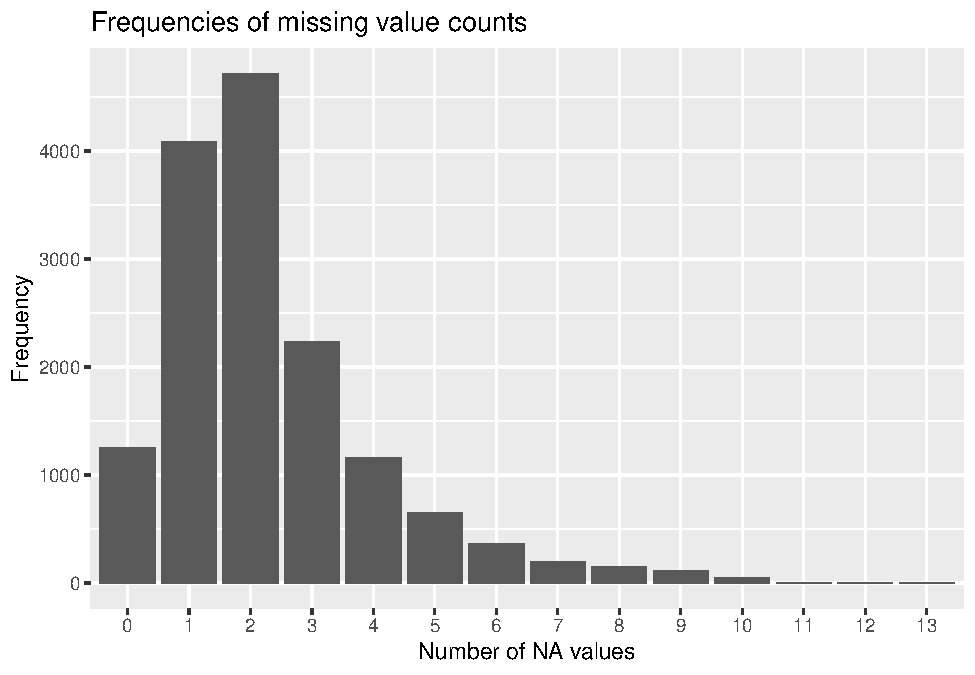
\includegraphics{hw4_files/figure-latex/unnamed-chunk-5-1.pdf}

\hypertarget{part-4}{%
\subsubsection{Part 4}\label{part-4}}

\begin{Shaded}
\begin{Highlighting}[]
\KeywordTok{mean}\NormalTok{(sample)}
\end{Highlighting}
\end{Shaded}

\begin{verbatim}
## [1] -0.1655812
\end{verbatim}

\begin{Shaded}
\begin{Highlighting}[]
\KeywordTok{sd}\NormalTok{(sample)}
\end{Highlighting}
\end{Shaded}

\begin{verbatim}
## [1] 0.7641279
\end{verbatim}

\hypertarget{exercise-4}{%
\section{Exercise 4}\label{exercise-4}}

Create a new version of your \texttt{rhand} function called
\texttt{rhand\_rejected}. Instead of returning the sampled vaues, the
\texttt{rhand\_rejected} function should keep track of and return the
number of points that were rejected.

What percentage of points is typically rejected for your rejection
sampler? Use an average across multiple runs to get a more accurate
estimate.

\emph{Hint: The \texttt{replicate} function may be helpful for calling
\texttt{rhand\_rejected} repeatedly.}

\textbf{YOUR ANSWER GOES HERE:}

About \texttt{53\%} of the points are typically rejected.

\begin{Shaded}
\begin{Highlighting}[]
\NormalTok{rhand\_rejected =}\StringTok{ }\ControlFlowTok{function}\NormalTok{(}\DataTypeTok{n =} \DecValTok{100}\NormalTok{) \{}
\NormalTok{   count =}\StringTok{ }\DecValTok{0}
\NormalTok{   iterations =}\StringTok{ }\DecValTok{0}
   \ControlFlowTok{while}\NormalTok{ (count }\OperatorTok{\textless{}}\StringTok{ }\NormalTok{n) \{}
\NormalTok{      iterations =}\StringTok{ }\NormalTok{iterations }\OperatorTok{+}\StringTok{ }\DecValTok{1}
\NormalTok{      x =}\StringTok{ }\KeywordTok{runif}\NormalTok{(}\DecValTok{1}\NormalTok{, }\FloatTok{{-}1.6}\NormalTok{, }\FloatTok{1.6}\NormalTok{)}
\NormalTok{      y =}\StringTok{ }\KeywordTok{runif}\NormalTok{(}\DecValTok{1}\NormalTok{, }\DecValTok{0}\NormalTok{, }\FloatTok{3.5}\NormalTok{)}
      \ControlFlowTok{if}\NormalTok{ (y }\OperatorTok{\textgreater{}}\StringTok{ }\KeywordTok{dhand}\NormalTok{(x)) \{}
\NormalTok{         count =}\StringTok{ }\NormalTok{count }\OperatorTok{+}\StringTok{ }\DecValTok{1}
\NormalTok{      \}}
\NormalTok{   \}}

\NormalTok{   iterations }\OperatorTok{{-}}\StringTok{ }\NormalTok{n}
\NormalTok{\}}
\NormalTok{n =}\StringTok{ }\DecValTok{1000}
\KeywordTok{mean}\NormalTok{(}\KeywordTok{replicate}\NormalTok{(}\DecValTok{100}\NormalTok{, }\DecValTok{1} \OperatorTok{{-}}\StringTok{ }\NormalTok{n }\OperatorTok{/}\StringTok{ }\NormalTok{(n }\OperatorTok{+}\StringTok{ }\KeywordTok{rhand\_rejected}\NormalTok{(n))))}
\end{Highlighting}
\end{Shaded}

\begin{verbatim}
## [1] 0.5373334
\end{verbatim}

\end{document}
